\subsection{Lifted \strips (LS) Transformer}
\label{sec:ls-transformer}

To predict whether a domain action $a_i$ is applicable, the LS Transformer checks whether all its ground preconditions hold. For each precondition $p(\mathbf{o})$, its truth value is determined by the most recent preceding domain or initialization action that affects it: an add
effect makes it true, while a delete effect makes it false.
% To determine whether an action $a_i$ is applicable after an action sequence $\tau$ from a given initial state, we check whether all its ground preconditions hold. For each precondition $p(\mathbf{o})$, its truth value is determined by the most recent preceding action $a_j \in \tau$, with $j<i$, that affects it: an add effect makes it true, while a delete effect makes it false.
The LS Transformer implements this computation through structured self-attention, extending the \strips Transformer of \citet{nunez2026strips} to the lifted setting. It is based on the \brasp program in
Appendix~\ref{app:brap-program} and described in detail in
Appendix~\ref{app:ls-transformer-extended}.

The LS Transformer has a single self-attention layer with one head per hidden predicate $p\in\mathcal{P}'$.
The number and arities of the hidden predicates are hyperparameters and need not match the ground-truth set $\mathcal{P}$. Each head checks preconditions involving its predicate.

For each predicate $p\in\mathcal{P}'$, action schema $\alpha\in A$, and valid pattern $\rho$, the parameters $\theta$ contain three scalars
$\theta^{\mathrm{pre}}_{p,\alpha,\rho}$,
$\theta^{\mathrm{eff}}_{p,\alpha,\rho}$, and
$\theta^{\mathrm{del}}_{p,\alpha,\rho}$.
These are mapped to relaxed values
$q_{p,\alpha,\rho},k_{p,\alpha,\rho},v_{p,\alpha,\rho}\in[0,1]$,
encoding whether the lifted atom $p(x_{\rho_1},\ldots,x_{\rho_r})$ is a precondition, an effect, and a delete rather than an add effect, respectively. These relaxations enable end-to-end differentiable learning and are binarized for inference. For binary values, $q=1$ specifies a precondition, while $k=1$ specifies an effect whose sign is determined by $v$: $v=0$ denotes an add effect and $v=1$ a delete effect.

The auxiliary actions from Section~\ref{sec:learning-task} use fixed parameters: \texttt{init-}$p$ and \texttt{goal-}$p$ are tied to the same hidden
predicate through the identity pattern, while \texttt{init-start} resets all atoms to false.

%The LS Transformer also encodes the auxiliary actions introduced in Section~\ref{sec:learning-task}. For a predicate $p$ of arity $r$, $\texttt{init-}p$ has no preconditions and $p(x_1,\ldots,x_r)$ as its single add effect, while $\texttt{goal-}p$ has no effects and the same atom as its single precondition. Both occurrences use the identity pattern $\rho=(1,\ldots,r)$. The special \texttt{init-start} action is encoded as setting every ground atom to false.

Each ground action $a_i=\alpha_i(\mathbf{o}_i)$ has a fixed binary embedding
containing one-hot encodings of its schema and object arguments.
Pattern-specific projections constructed from $\theta$ yield the scores
\begin{align}
S_{p,\rho,\sigma}(i,j)
&=
q_{p,\alpha_i,\rho}\,
k_{p,\alpha_j,\sigma}\,
\mathbb{I}\!\left[
\mathbf{o}_i^\rho=\mathbf{o}_j^\sigma
\right],
\label{eq:scores}
\end{align}
where $\mathbf{o}_i^\rho$ is the object tuple selected by $\rho$.
For binary parameters, the score is $1$ exactly when $(p,\rho)$ is a
precondition of $\alpha_i$, $(p,\sigma)$ is an effect of $\alpha_j$, and both
patterns ground to the same atom.

%Each ground action $a_i=\alpha_i(\mathbf{o}_i)$ is represented by a fixed binary embedding containing one-hot encodings of its schema and object arguments. Linear projections constructed from $\theta$ produce queries, keys, and values, with the queries and keys yielding the self-attention scores
%\begin{align}\label{eq:scores}
%S_{p,\rho,\sigma}(i,j)
%&=
%q_{p,\alpha_i,\rho}\,
%k_{p,\alpha_j,\sigma}\,
%\mathbb{I}\!\left[
%\mathbf{o}_i^\rho=\mathbf{o}_j^\sigma
%\right],
%\end{align}
%where $\mathbf{o}_i^\rho$ denotes the object tuple selected by $\rho$ from $\mathbf{o}_i$. For binary parameters, this score is $1$ iff $q_{p,\alpha_i,\rho}=1$, so $\alpha_i$ has the precondition specified by $(p,\rho)$; $k_{p,\alpha_j,\sigma}=1$, so $\alpha_j$ has the effect specified by $(p,\sigma)$; and $\mathbf{o}_i^\rho=\mathbf{o}_j^\sigma$, so the precondition and effect refer to the same ground atom.

Strict future masking restricts attention to $j<i$.
For each precondition pattern $\rho$, stick-breaking normalization accounts for all effect patterns $\sigma$ at every preceding position. With binary parameters, it selects the most recent effect on the corresponding
ground atom, matching \strips semantics.

%Strict future masking restricts attention to $j<i$.
%Then, stick-breaking normalization is applied separately for each precondition pattern $\rho$. With binary parameters, it selects the most recent preceding effect on the corresponding ground precondition $p(o_i^\rho)$. This encodes an inductive bias aligned with \strips semantics.

Combining the normalized weights with $V_{p,\sigma}(j)=v_{p,\alpha_j,\sigma}$ yields the violation score
$Y_{p,\rho}(i)$. For binary parameters, this score is $1$ exactly when $(p,\rho)$ specifies a precondition of $a_i$ and the corresponding ground atom is false.
%The normalized attention scores are combined with the values $v_{p,\alpha_j,\sigma}$ to obtain $Y_{p,\rho}(i)$.
%For binary parameters, $Y_{p,\rho}(i)$ is a violation indicator: it is $1$ exactly when $(p,\rho)$ specifies a precondition of $a_i$ and the corresponding ground atom is false.
%For binary parameters, $Y_{p,\rho}(i)$ is $0$ when the ground precondition $p(\mathbf{o}_i^\rho)$ is true (i.e., satisfied) and $1$ otherwise.
A continuous OR gives the action-level inapplicability score
\[
Y_\theta(i)
=
1-\prod_{p\in\mathcal{P}'}\prod_{\rho}
\bigl(1-Y_{p,\rho}(i)\bigr),
\]
where the second product ranges over valid patterns.
For binary parameters, $Y_\theta(i)=1$ iff at least one precondition is false,
so $a_i$ is applicable iff $Y_\theta(i)=0$.
%Next, we perform aggregation with a continuous OR operation, to determine action applicability:
%\[ Y_\theta(i) = 1-\prod_{p\in\mathcal{P}'}\prod_{\rho} \bigl(1-Y_{p,\rho}(i)\bigr). \]
%$Y_\theta(i)=1$ iff one or more preconditions are false. Therefore, $a_i$ is applicable iff $Y_\theta(i)=0$.

The parameters $\theta$ are indexed by hidden predicates, action schemas, and patterns, but not by object identities or the number of objects. Changing the object set changes only the fixed action embeddings and projection matrices, allowing the same learned parameters to be instantiated on traces with different numbers of objects.

%Finally, we note that the transformer parameters $\theta$ are lifted: they depend on the hidden predicates $\mathcal{P}'$ and action schemas $A$, but not on the objects $O$ appearing in the traces. The same parameters can therefore be instantiated on traces with more objects than those seen during training.


\iffalse
    \noindent
    \begin{minipage}[t]{0.53\textwidth}
    \vspace{0pt}
        \centering
        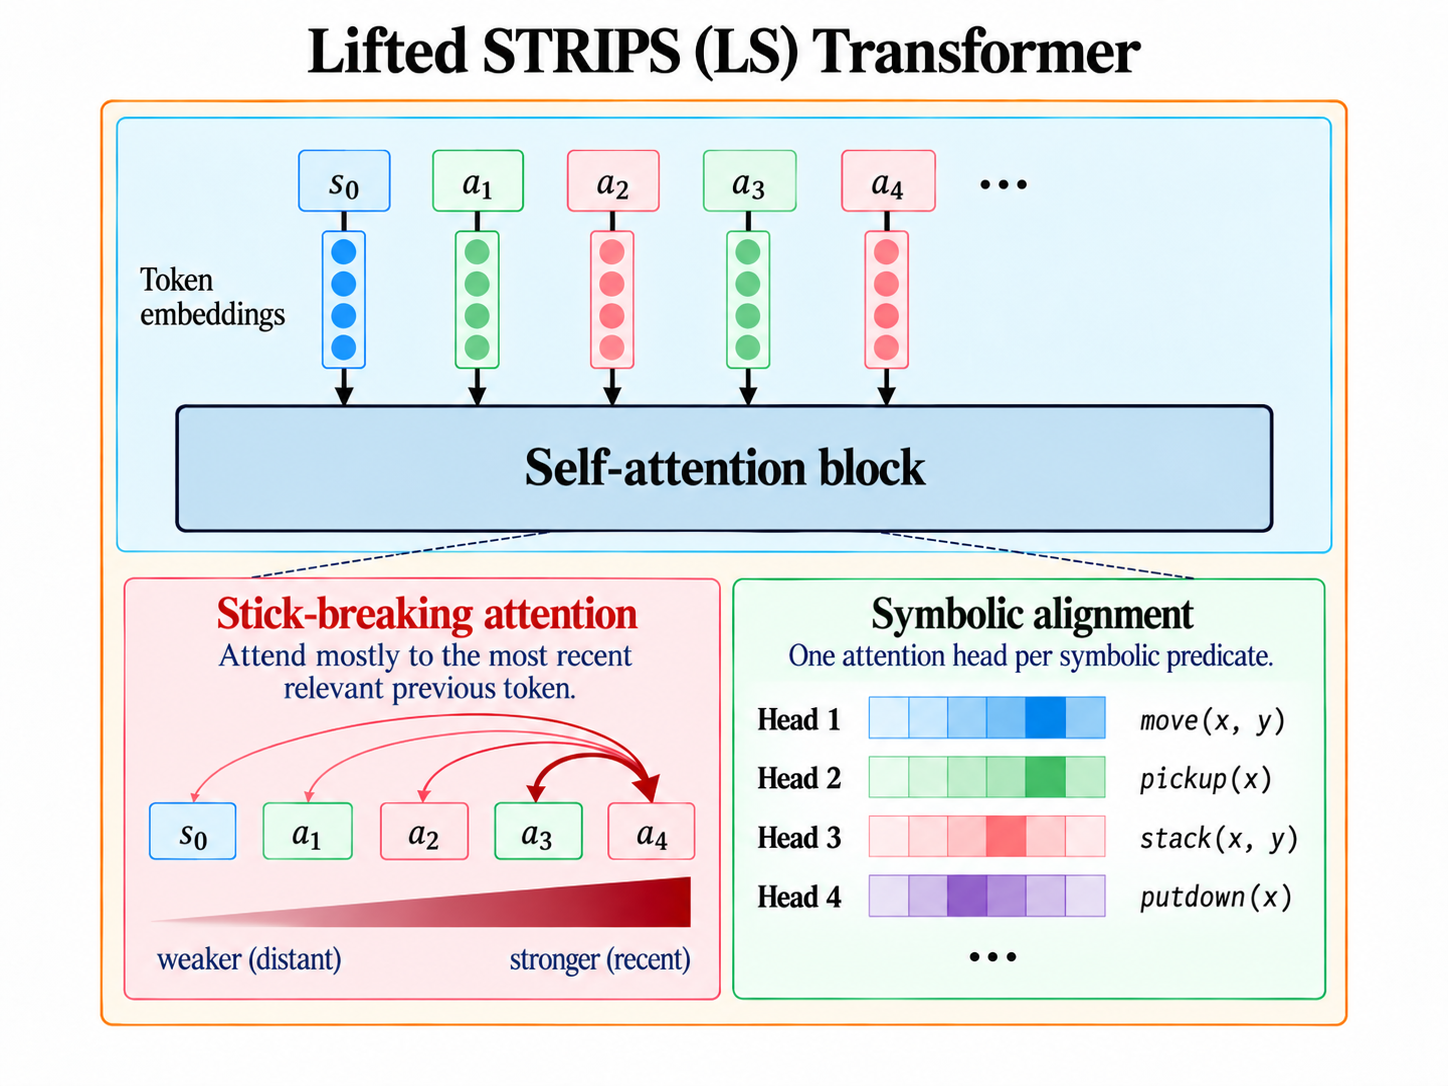
\includegraphics[width=\linewidth]{LS_transformer.png}
        \captionof{figure}{Architecture of the Lifted \strips Transformer.}
        \label{fig:ls-transformer}
    \end{minipage}
    \hfill
    \begin{minipage}[t]{0.48\textwidth}
    \vspace{0pt}
    
    \end{minipage}
\fi





\subsection{Lifted Stick-Breaking (LB) Transformer}
\label{sec:lb-transformer}
The LB Transformer generalizes the SB Transformer of
\citet{nunez2026strips} to the lifted \strips setting.
It is a decoder-style Transformer with stick-breaking
attention~\citep{tan2025scaling}, strict future masking, and no positional encodings. Unlike the LS Transformer, its parameters do not explicitly represent predicates, preconditions, or effects.
%The LB Transformer  the SB Transformer of \citet{nunez2026strips} to the lifted \strips{} setting. Unlike the LS Transformer, its parameters do not explicitly represent predicates, preconditions, or effects. It follows a decoder-style Transformer architecture, replacing softmax with stick-breaking attention~\citep{tan2025scaling}, using strict future masking and no positional encodings.

Each ground action
$a_i=\alpha_i(o_{i,1},\ldots,o_{i,k_i})$ is encoded as
\[
\alpha_i,\;o_{i,1},\;\ldots,\;o_{i,k_i},\;\texttt{<sep>}.
\]
Concatenating these sequences yields the trace representation.
Action-schema and \texttt{<sep>} tokens use learned embeddings, while object
tokens use randomized, non-learnable embeddings.
Each action label is associated with its trailing \texttt{<sep>} token.
A linear output layer applied to its final contextual representation yields
$y_\theta(i)\in[0,1]$, the predicted probability that $a_i$ is inapplicable
given the preceding actions.

%Each ground action $a_i=\alpha_i(o_{i,1},\ldots,o_{i,k_i})$ is encoded as the token sequence $\alpha_i,\;o_{i,1},\;\ldots,\;o_{i,k_i},\;\texttt{<sep>}$. Concatenating these sequences yields the input representation of the trace. Action-schema and \texttt{<sep>} tokens use standard learnable embeddings, whereas objects use randomized, non-learnable embeddings.
%Each action's label and prediction are associated with its following \texttt{<sep>} token. The final contextual representation of this token produces $y_\theta(i)\in[0,1]$, the predicted probability that $a_i$ is inapplicable given the preceding actions in the trace.


For each presentation of a trace, every object $o$ is assigned a distinct embedding $r(o)\in\{-1,+1\}^{d_{\mathrm{model}}}$, sampled uniformly without
replacement. 
%For each trace, every object $o$ is assigned an embedding $r(o)\in\{-1,+1\}^{d_{\mathrm{model}}}$, with each coordinate sampled independently and uniformly.
The same embedding is reused for all occurrences of $o$ within that trace, allowing the transformer to recognize when arguments of different actions refer to the same object. Object embeddings are resampled whenever a trace is sampled, encouraging the transformer to learn lifted operations that are invariant under object renamings. 
The representation supports up to
$2^{d_{\mathrm{model}}}$ distinct objects per trace.
Because these embeddings are generated on demand rather than selected from a
learned vocabulary, the same network can process traces with more objects than
those seen during training.